
\iffalse
Features  
\begin{itemize}
	\item Qualitative representation - states and transitions
	\item State identification services:
	\begin{itemize}
		\item State details and attribute highlighting - histograms + attribute colors
		\item \lstopar{Timeline + parallel coordinates \cite{parcoords} - when do states occur in time}
		\item \lstopar{Coloring states based on attributes}
		\item Decision trees + rule extraction - Explanation of states
		\item Automatic name generation
		\item Zooming into a state + showing paths from a state
	\end{itemize}
\end{itemize}
\fi

After registering, the user is presented with a dashboard, where they can organize their models.
If they wish to create a new model, they have to upload a CSV file with the dataset they would
like to visualize. They are then taken through a configuration form, where they select attributes,
clustering method, aggregation strategy and attributes used to model transitions. When completing
the form, their new model is constructed. The construction time varies depending on the size of 
their dataset and configuration. We conducted and experiment to test the performance of our \lstopar{methodology},
presented in section \ref{sec:implementation}.

Once constructed, a StreamStory model is displayed using a three panel user interface, an example of
which is shown in Figure \ref{fig:teaser} \lstopar{[TODO teaser reference not appearing]}. As mentioned
in Section \ref{sec:introduction} \lstopar{[TODO reference not showing]}, we summarize the model in a qualitative manner using states and 
transitions, where we associate each state with a circle and each transition with an arrow on the 
central panel. The size of a state is calculated from the associated entry in the stationary distribution
and is proportional to the fraction of time the system spends in the state. The thickness of each arrow
is proportional to the associated transition probability. When using the model as a
monitoring tool, the current state (green) and the most likely future states (blue)
are highlighted. The current state is determined by assigning the sample to its nearest 
centroid, as presented in Section \ref{sec:multiscale-implementation}, and is updated in real-time as
data arrives into the system.

When first opening the user interface, the model is presented on a coerce scale with only a handful
of states. Users can then explore the model by either traversing the scales using the zoom 
function, isolate and explore individual states using the "Zoom Into" function, \lstopar{or explore the 
graph as a tree using the "Show Path" function}.

A graph with states and transitions is not very informative by itself. Therefore we offer several 
visualization services which assist users identifying the meaning of states. These range from automatic
state naming, state histograms, attribute highlighting and timeline histograms to decision trees
which visualize the states' properties in a hierarchical manner and \lstopar{extracted rules}.
These services are shown when the user clicks on a state and thereby selects it. They will be 
explained in the following subsections.

\subsection{Histograms and Attribute Highlighting}

As the most basic exploratory tool we show the distribution of data inside each state in the form of a histogram.
When clicking on a state, the histograms of all the attributes are shows in the right-side panel like in
Figure \ref{fig:teaser} \lstopar{[teaser not showing!]}. Additionally to the standard histogram, we also 
provide a context, by showing the global distribution of the attribute in the background.

To assist the users to distinguish between states, we highlight each attribute either green of red.
The color is chosen based on how typical the attribute is for the state. For example, a bright green
value suggests that the attribute has a higher value in this state compared to other states, while
a bright red color suggests, this value is low compared to other states. An example of attribute 
highlighting can be seen in Figure \ref{fig:example-naming-histogram}.

The color is calculated in the initialization step by first classifying all the samples assigned to this state 
against samples assigned to other states using a logistic regression model. \lstopar{The features used in the 
classification are all the dimensions of the input signal, which correspond to all the attributes.}
The final color is determined by extracting weights from the models and associating positive weights
with green color and negative with red.

The users can also view the distribution of attributes across states, by selecting a specific attribute.
When doing so, the states are recolored based on the value of the selected attribute - green indicates
a high value, while red indicates a low value.

\subsection{Automatic State Labeling}

Looking at graphs by itself is not very informative. Although representing the system as states and 
transitions gives insight into the dynamics of the system, it fails to provide a comprehensive summary 
of the dataset. \lstopar{Indeed, our experiments showed first time users were quite confused when viewing
our model with unlabeled states and had difficulty executing even the simplest tasks like finding
states with high temperature in example \ref{sec:experiments-weather}}.

To overcome this issue, an automatic, data-driven, naming service was implemented. The service labels
states based on the inner-state attribute distributions by concatenating the most outlying attribute
with a discrete level, ranging from: lowest, low to high and highest.

Both the attribute and the level used in the label are computed by comparing the inner-state attribute
distributions to the global attribute distributions. The attribute selected by the naming process is
the one with the lowest $p$-value of the inner-cluster $40$-th and $60$-th percentile. The level is
then determined according to the $p$-value. If the $p$-value is below $0.12$ the attribute is labeled
as lowest or highest, while is the $p$-value is below $0.25$ it is labeled low or high. If none of the
attributes achieve a $p$-value of $0.25$ the state is labeled as a mean state. An example of an automatic
label, along with the associated inner-state and global histogram is shown in Figure \ref{fig:example-naming}.

\begin{figure}[h!]
	\centering
	\begin{subfigure}{.48\columnwidth}
	  	\centering
	  	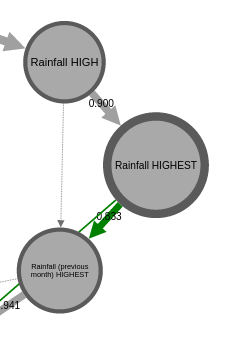
\includegraphics[width=0.7\columnwidth]{example-state-naming}
  		\caption{\label{fig:example-naming-label}\lstopar{TODO}}
	\end{subfigure}
	\begin{subfigure}{.48\columnwidth}
	  	\centering
	  	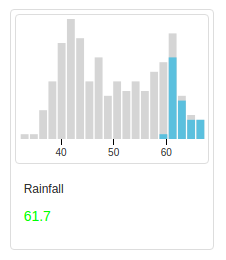
\includegraphics[width=\columnwidth]{example-state-naming-histogram}
	  	\caption{\label{fig:example-naming-histogram}\lstopar{TODO}}
	\end{subfigure}
	\caption{\lstopar{[TODO]}}
	\label{fig:example-naming}
\end{figure}

\iffalse
In order to assist the user in identifying the meaning of states, the system provides automatic default
state names, based on the distribution of attributes in the state. Each state is given a default name
by combining its most outstanding attribute with a discrete level: LOWEST, LOW, HIGH or
HIGHEST.

The attribute and the level are chosen by comparing its distribution inside the state to the global
distribution in all the states through histograms. This is achieved by first computing the percentiles
of the global distribution. The $40^{th}$ percentile is then computed for the state distribution and
compared against the global distribution. If this percentile lies below the $25^{th}$ or $12^{th}$
percentile, the state is marked with LOW or LOWEST respectively. The final name is chosen according
to the attribute which lies in the lowest percentile.
\fi

\subsection{Decision Trees and Rule Extraction}

An alternate description of a state is generated through the induction of decision trees \cite{Witten:2005:DMP:1205860}. Decision
trees are classification models often used in domains such as medicine for their explanatory power.
When a decision tree is induced, a splitting attribute and cut value are chosen recursively by a
design time criteria. The user can then interpret the tree by traversing the path from the root 
to one of the leafs.

In our use case, we use decision trees as a tool for explaining states. We induce one tree for each
state by classifying the observations of the state against the observations of all other states,
obtaining a quantitative description of the state. We then extract rules from the decision tree,
providing a short summary of the state in the form of $A_i > t_i \cup A_j \in (t_{j_1}, t_{j_2}]$.

Figure \ref{fig:example-decision-tree-and-rule} show an example decision tree and extracted rules
from a state in the weather dataset presented in section \ref{sec:experiments-weather}.

\begin{figure}[h!]
	\centering
	\begin{subfigure}{.3\columnwidth}
	  	\centering
	  	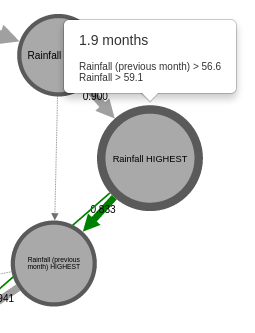
\includegraphics[width=\columnwidth]{example-rule}
  		\caption{\lstopar{TODO}}
  		\label{fig:example-rule}
	\end{subfigure}
	\begin{subfigure}{.68\columnwidth}
	  	\centering
	  	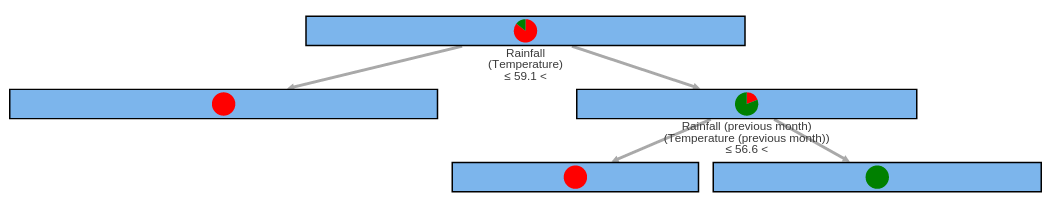
\includegraphics[width=\columnwidth]{example-decision-tree}
	  	\caption{\lstopar{TODO}}
	  	\label{fig:example-decision-tree}
	\end{subfigure}
	\caption{\lstopar{[TODO]}}
	\label{fig:example-decision-tree-and-rule}
\end{figure}

\iffalse
\subsection{Visual Assistance}

When a state becomes selected, the user interface presents the user with several visual aids which
assist them in identifying the states' meaning. The first of these aids is the timeline histogram
which shows the distribution of the states occurrence over time. An example is shown in Figure 
\ref{fig:time-hist}.

\begin{figure}[h!]
	\centering
	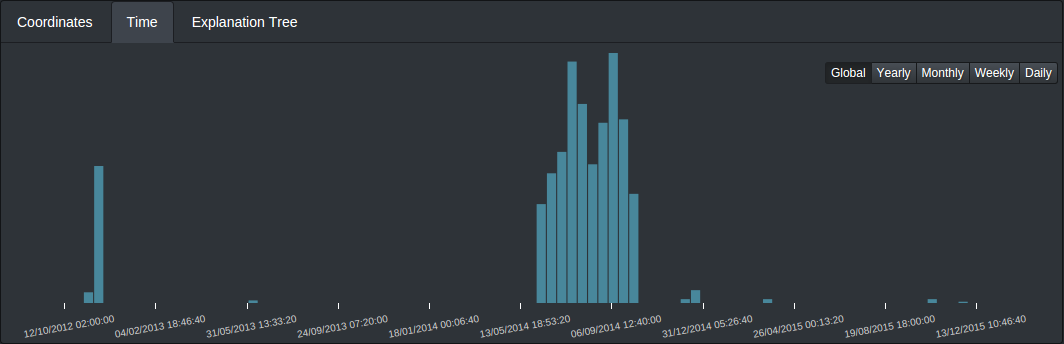
\includegraphics[width=\columnwidth]{timeline}
	\caption{[TODO example decision tree].}
	\label{fig:time-hist}
\end{figure}

[TODO histograms]
\fi
